%-----------------------------------------------------------------------------%
\chapter{\babEmpat}
\label{bab:4}
%-----------------------------------------------------------------------------%
% Bab ini menjelaskan tentang struktur dari \f{template} tugas akhir ini.
% Dengan memahami struktur \f{template}, pekerjaan Anda akan menjadi lebih terarah karena Anda tahu di mana Anda harus melakukan sesuatu.
This chapter explains the design and implementation of this research. The discussion consists of the application, Kubernetes, MCS with MCI geo-distributed cluster, Istio / ASM geo-distributed cluster, and performance testing.


%-----------------------------------------------------------------------------%

% \section{Application}
% \label{sec:application}

\section{Application}
% The application consists of a server and a database. The server is a REST API written in the Go programming language and is chosen as the programming language for the implementation of the server of its speed as well as language uniformity with Docker and Kubernetes. The database is a Redis instance, chosen for being lightweight and simple to use. The implementation of the server can be seen in the \code{main.go} file and the Redis implementation is used from the official Redis docker container and will be explained in \autoref{sec:kubernetes-implementation}.
% \lstinputlisting[language=Go, caption=Simple REST API written in Go, label=code:go]{assets/codes/main.go}

% \section{Application Infrastucture Design}
% \label{sec:applicationInfrastructureDesign}
There are two areas that were configured in the complete web application, the application server itself and the geo-distributed Kubernetes clusters. In the first step, we implemented the application itself. We chose a two-tiered application consisting of a server and a database tier for this research as it covers all the main components that were tested. The client tier is absent and is replaced by the Vegeta load testing tool. 

After the application design/architecture was configured, next are the application implementation details. First of all, the server is a REST API that communicates with a database and simply returns the cluster name of where the responding server is located. We wrote the server in the Go programming language for its speed as well as language uniformity with Docker and Kubernetes. Furthermore, its implementation can be seen in \code{main.go}\footnote{\url{https://github.com/jojonicho/skripsi/blob/master/server/main.go}}. Finally, it was containerized using Docker and uploaded to Docker Hub to be used by Kubernetes. In addition, we chose Redis as the database for its simplicity as well as being lightweight, an important aspect of web performance. The integration of Kubernetes inside of a development workflow creates a separation of concern between application development and infrastructure development, which allows for concurrent progress between the two different areas and is a big reason why Docker and Kubernetes are widely adopted.

The next step after application configuration was the geo-distributed clusters configuration consisting of MCS with MCI and Istio / ASM. First, in the MCS with MCI configuration, we deployed the server service as a MultiClusterService custom resource, which was routed by the MultiClusterIngress custom resource and allows cross-cluster communication. Following this, a virtual IP address was created, which uses a Google Cloud Load Balancer to route traffic to the nearest cluster. The infrastructure for the MCS with MCI geo-distributed Kubernetes clusters can be seen in \autoref{fig:infra-mcs-mci}.

\begin{figure}
	\centering
	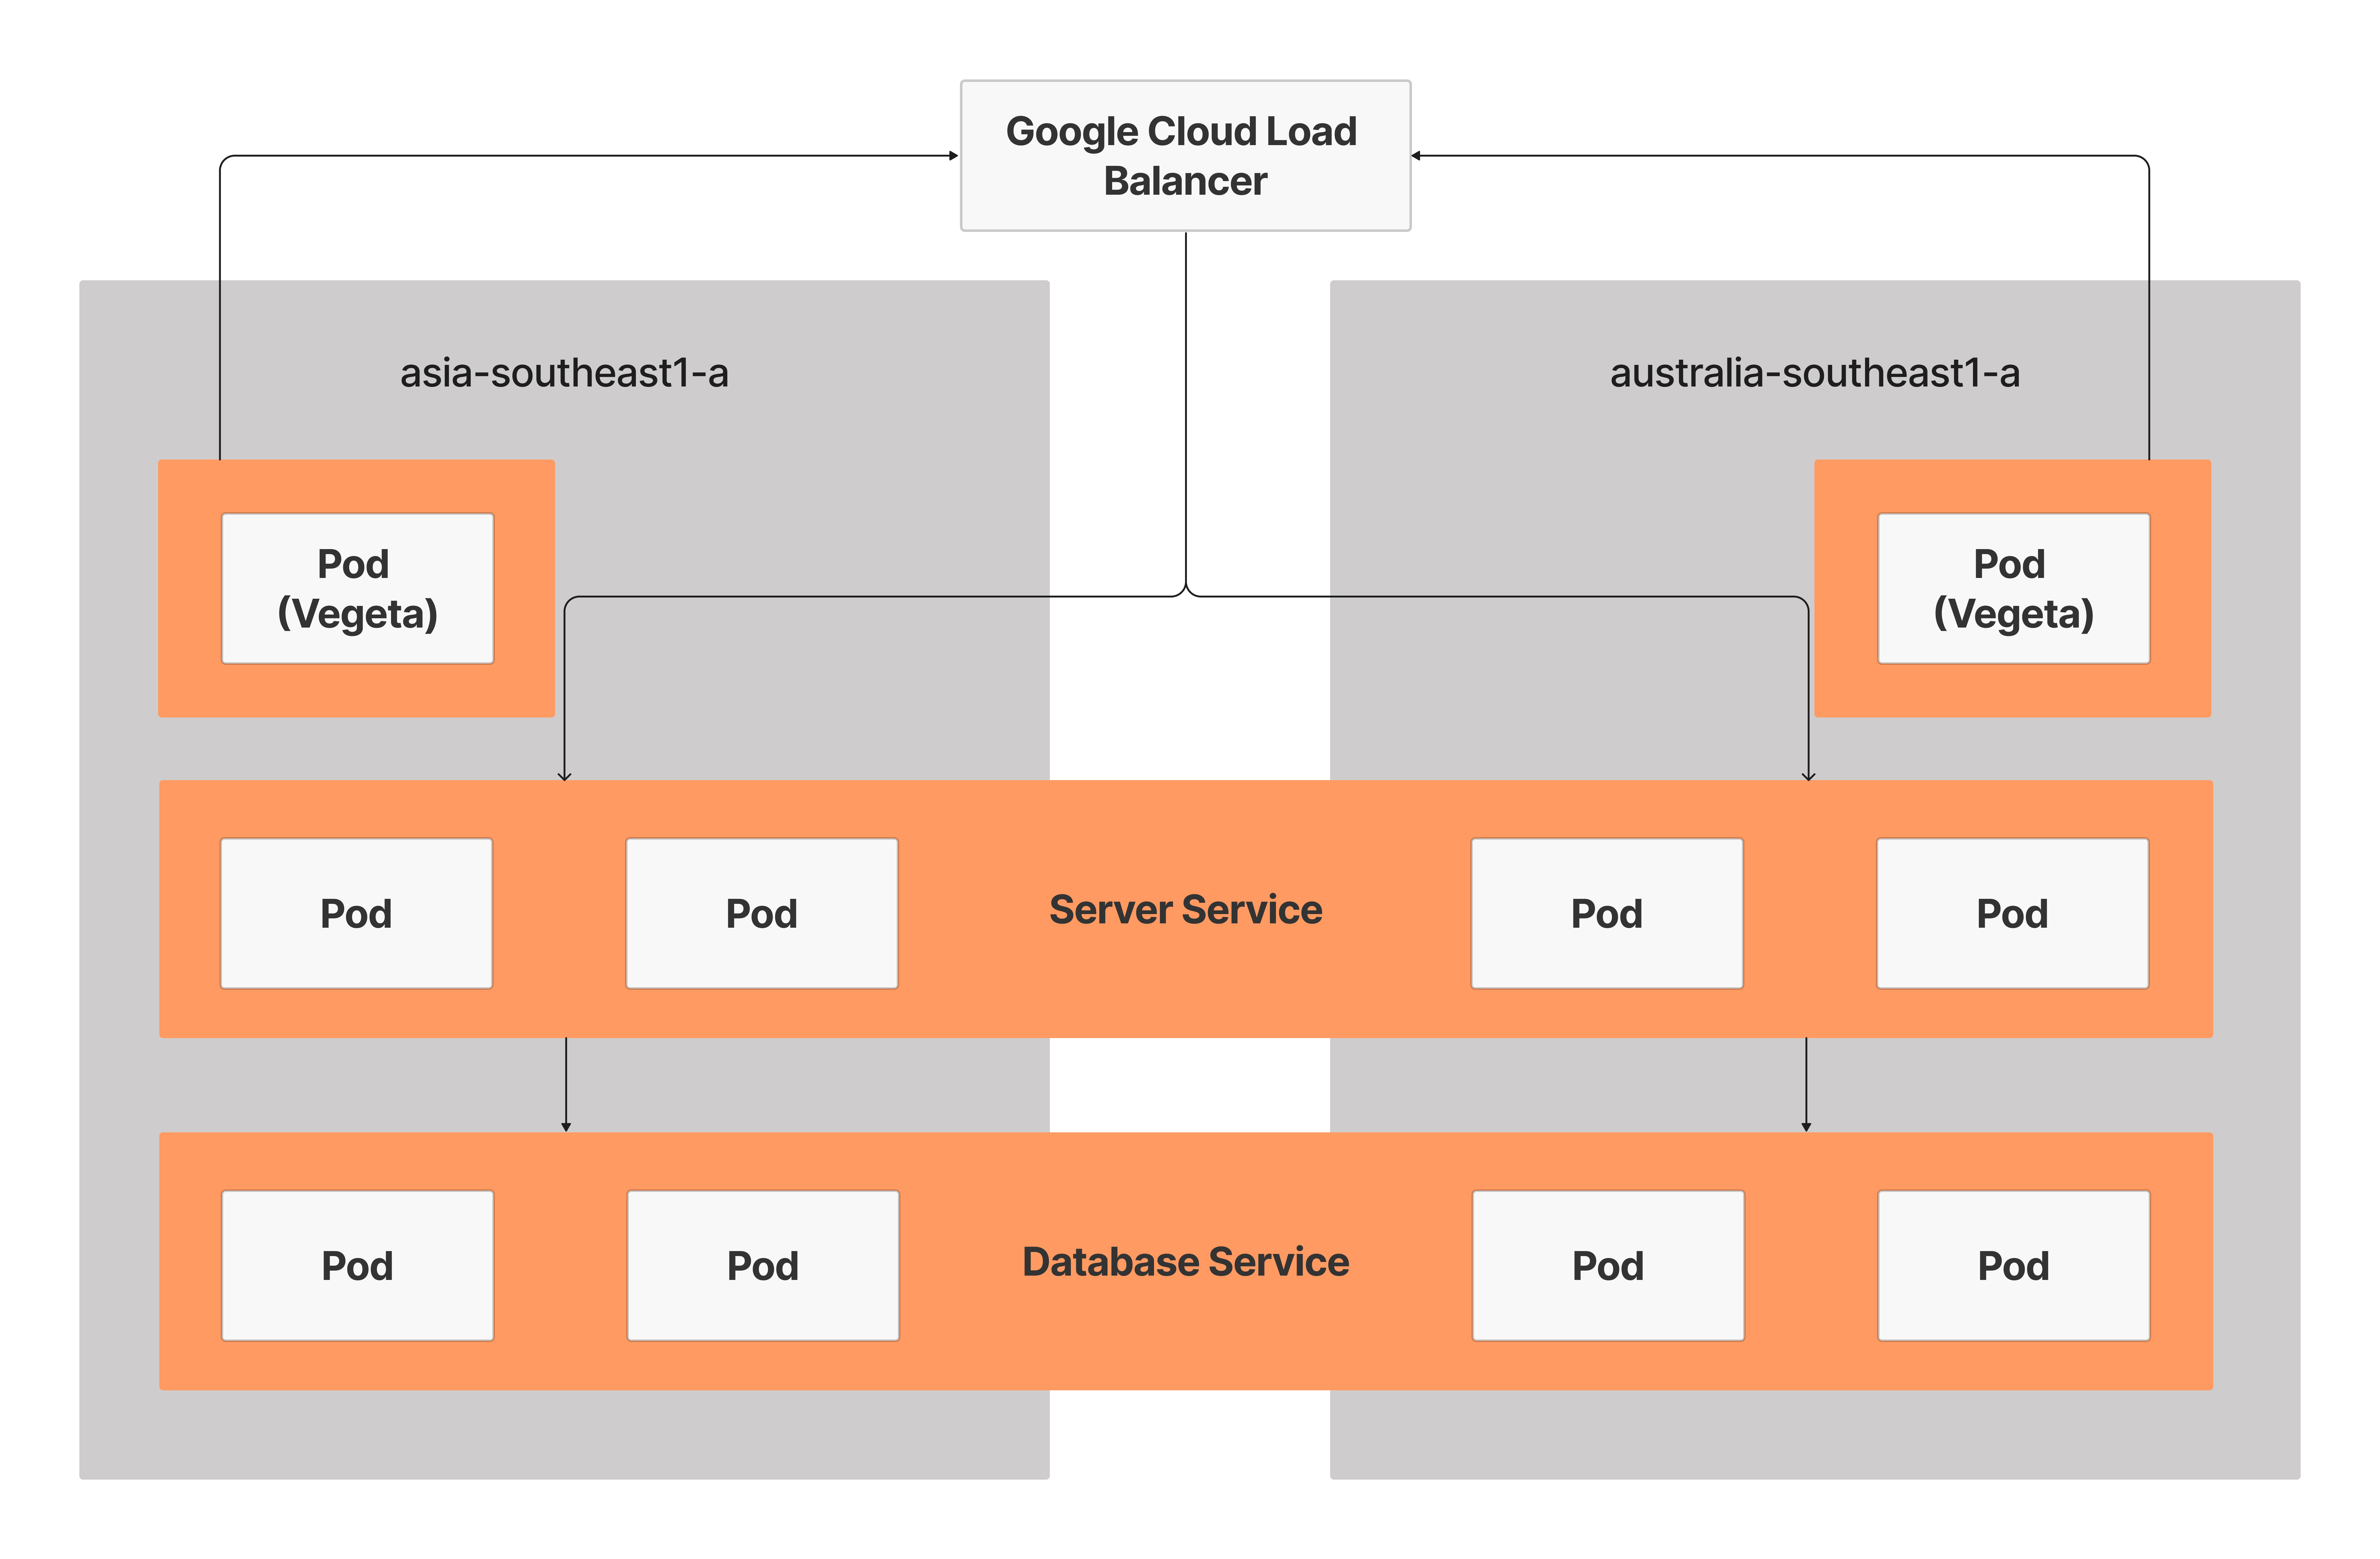
\includegraphics[width=1\textwidth]{assets/diagrams/infra-mcs-mci.png}
	\caption{Geo-distributed Kubernetes clusters infrastructure on the MCS with MCI configuration.}
	\label{fig:infra-mcs-mci}
\end{figure}

% each cluster is installed with Istio control and data plane which
% Next, in the Istio / ASM configuration, installing Istio control and data plane in each cluster enables automatic envoy proxy injection to each pod. We then deploy the DestinationRule resource to configure locality load balancing, which routes traffic to the nearest cluster. Following this, we deployed the Vegeta load testing pod in every region to simulate a request call from a specific region. We decided to use the server layer as a data layer, which is a server connected to each database instance as a solution to the problem of the database layer not being able to be load balanced directly as the database instance is needed on the server runtime. Lastly, the Istio / ASM geo-distributed Kubernetes clusters' infrastructure can be seen in \autoref{fig:infra-istio}.

Next, in the Istio / ASM configuration, we installed the Istio control and data plane in each cluster, which enabled automatic envoy proxy injection to each pod. We then deployed the DestinationRule resource to configure locality load balancing, which routes traffic to the nearest cluster. Following this, we deployed the Vegeta load testing pod in every region to simulate a request call from a specific region. We decided to use the server layer as a data layer, which is a server connected to each database instance because it is not possible to load-balance the database layer directly, as the database instance is a run-time dependency. Lastly, the Istio / ASM geo-distributed Kubernetes clusters' infrastructure can be seen in \autoref{fig:infra-istio}.

% To handle the problem of the database layer not being able to be load balanced directly, as a result of the database instance being needed on the server runtime, a problem that can be handled by having a dedicated data layer which is a server for each database instance

\begin{figure}
	\centering
	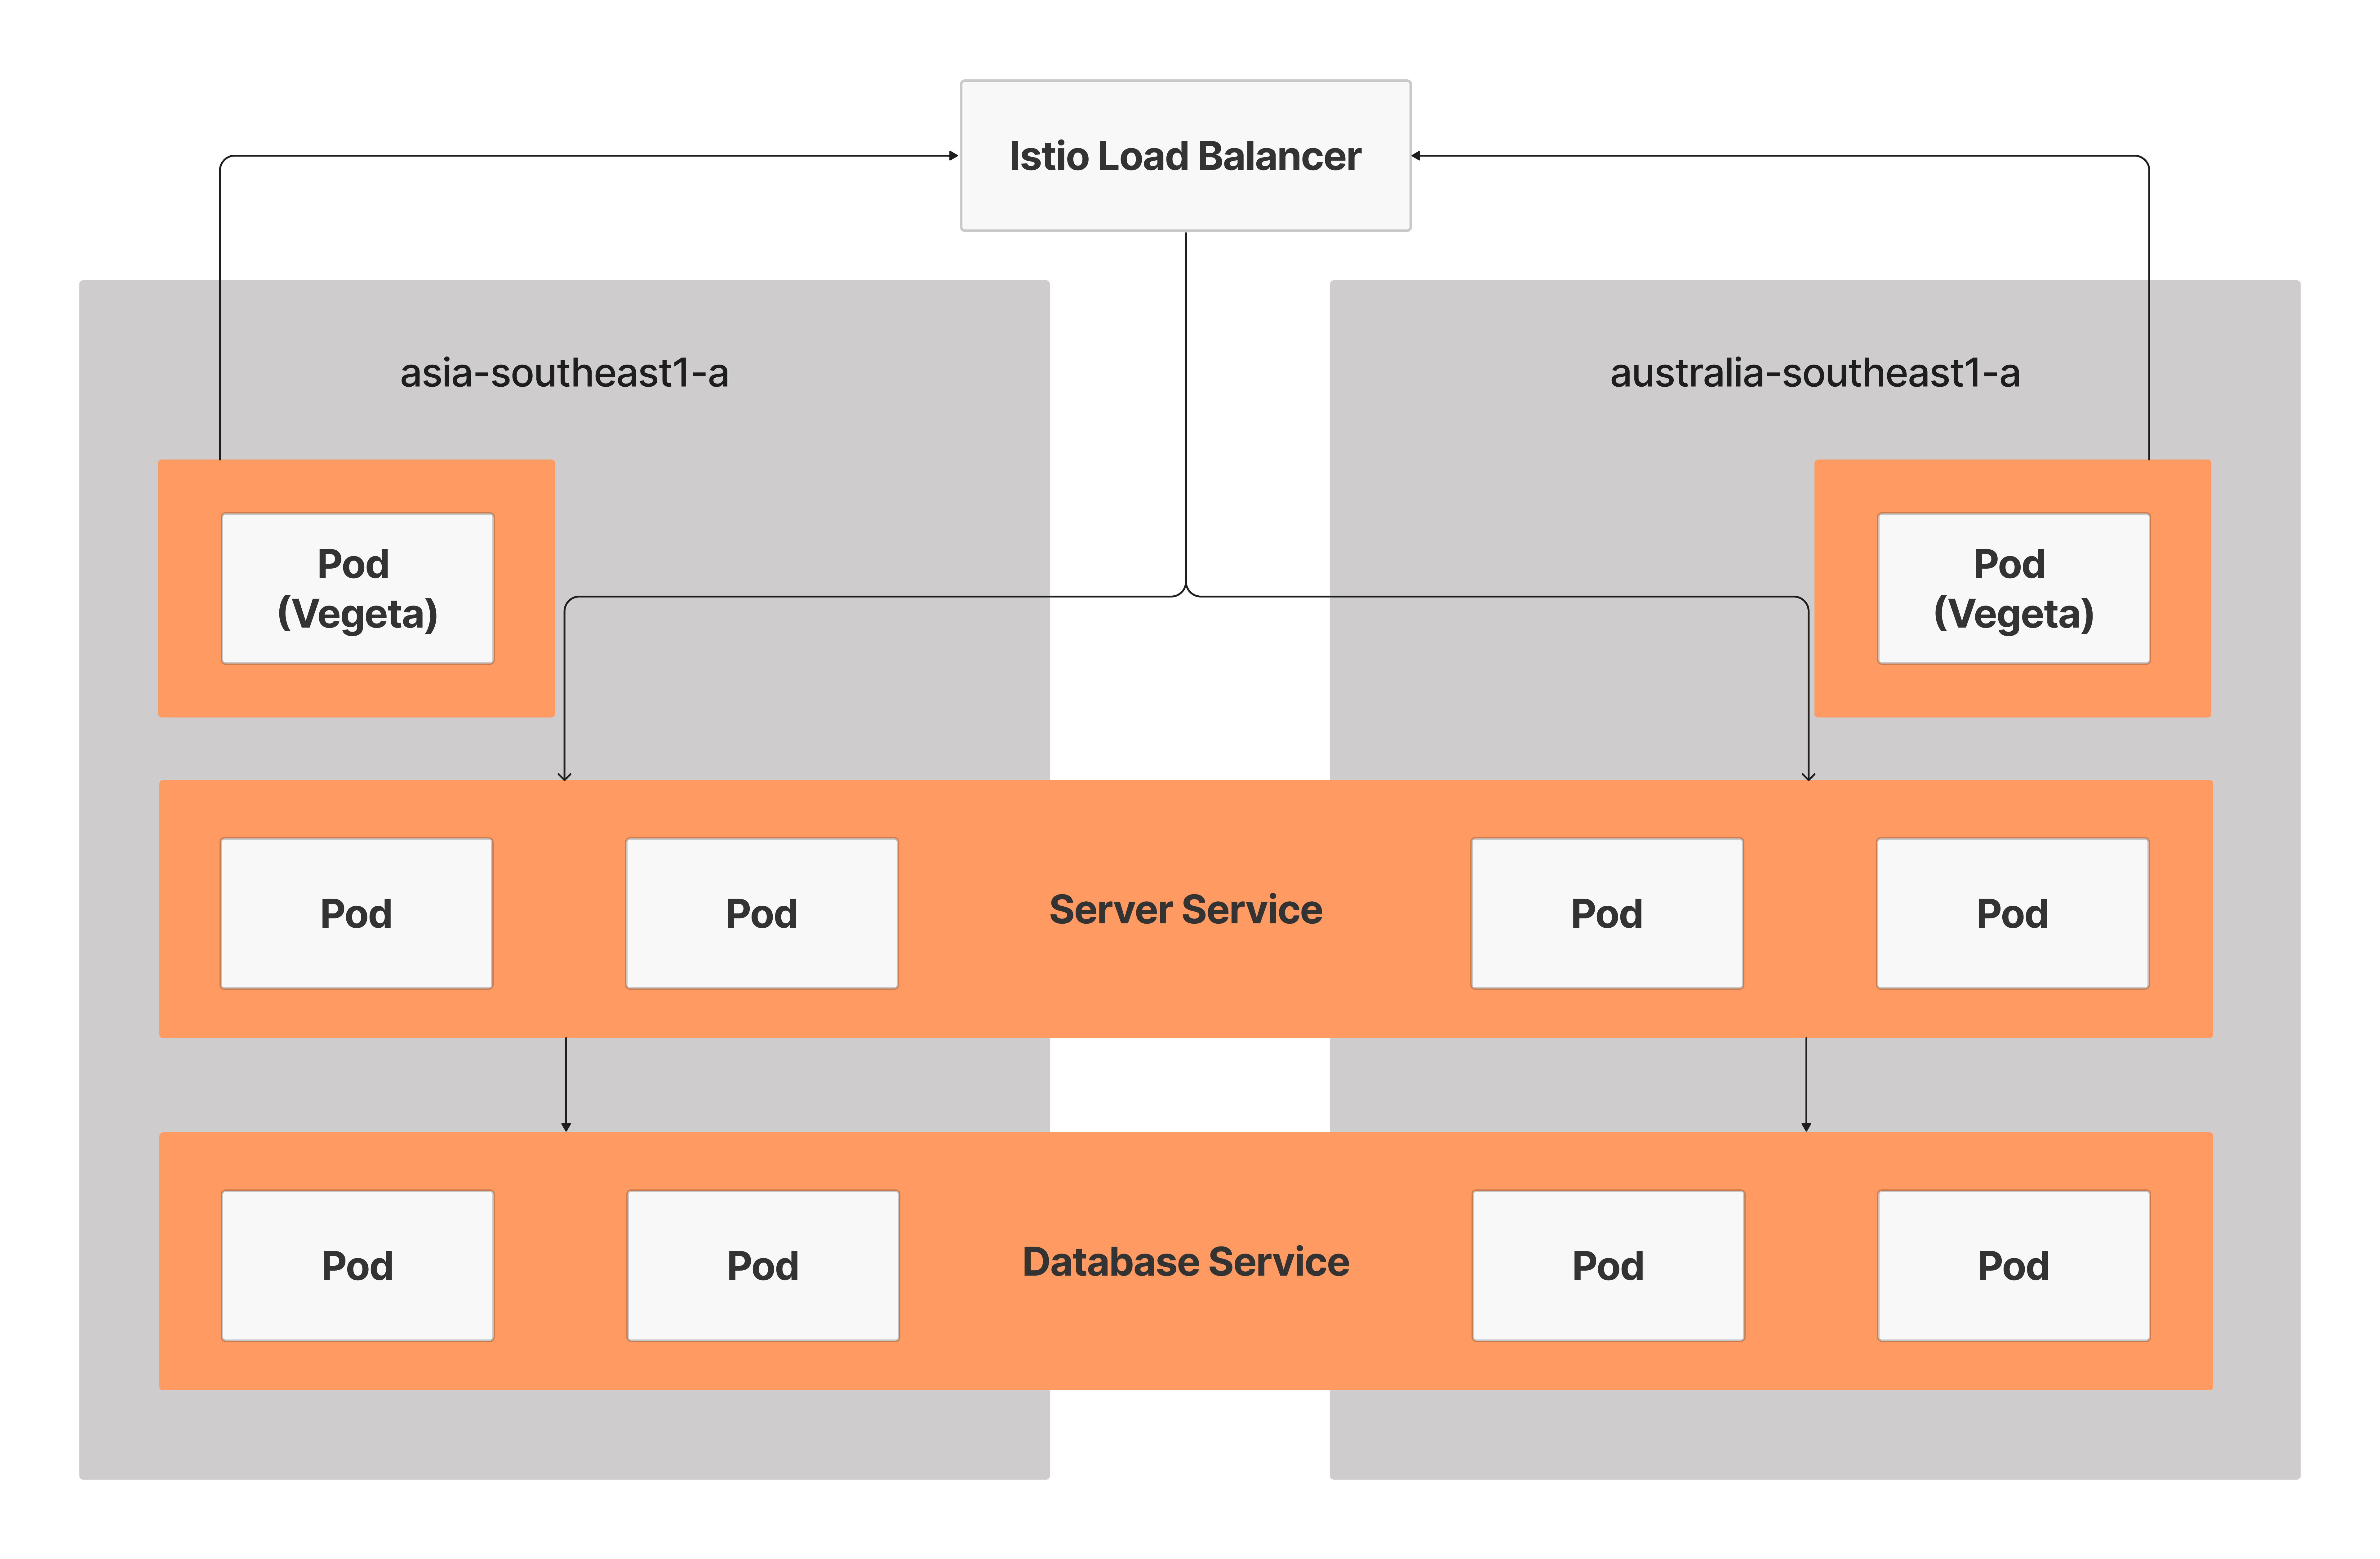
\includegraphics[width=1\textwidth]{assets/diagrams/infra-istio.png}
	\caption{Geo-distributed Kubernetes cluster infrastructure on Istio / ASM configuration.}
	\label{fig:infra-istio}
\end{figure}

\subsection{Kubernetes}
\label{sec:kubernetes-implementation}
% The Kubernetes implementation consists of YAML files which are applied using the \code{kubectl} command-line interface on Google Kubernetes Engine clusters. The Kubernetes implementation for the application can be seen in \autoref{code:client-yaml}, \autoref{code:server-yaml}, and \autoref{code:redis-yaml}
Besides implementing the application, configuring and implementing a Kubernetes architecture was another important step to successfully deploy a geo-distributed cluster web application. Kubernetes implementation and configuration were done through YAML files, which we then applied using the \code{kubectl} command-line interface on Google Kubernetes Engine clusters, where its implementation can be seen in the GitHub repository\footnote{\url{https://github.com/jojonicho/skripsi}}. One of the main selling points of Kubernetes is its networking features, which allow services to communicate with each other and conveniently map each service name defined in the metadata to a URL value that can be provided as an environment variable. For example, to connect the \code{ta-server} service with the \code{ta-redis} service, simply provide \code{ta-redis-service} inside of the server YAML file\footnote{\url{https://github.com/jojonicho/skripsi/blob/master/server.yaml}}, and the redis URL can be accessed inside of the server application as an environment variable.

% is convenient because the service name defined in the metadata section of a service can also be used as a URL mapping to be provided as an environment variable

% \lstinputlisting[language=Yaml, caption=Service and Deployment configuration for ta-client application, label=code:client-yaml]{assets/codes/client.yaml}

% \lstinputlisting[language=Yaml, caption=Service and Deployment configuration for ta-server application, label=code:server-yaml]{assets/codes/server.yaml}

% \lstinputlisting[language=Yaml, caption=Service and Deployment configuration for ta-redis application, label=code:redis-yaml]{assets/codes/redis.yaml}

% \section{Google Kubernetes Engine Cluster Implementation}
% \label{sec:kubernetes-cluster-configuration}
% % \subsection{Kubernetes}

All of the Kubernetes YAML files were applied on Google Kubernetes Engine clusters. Each of the clusters was created using the \code{gcloud} command as shown in \autoref{code:1-create-cluster-se-asia-sh} and each having the configuration shown in \autoref{table:cluster-configuration}.

\vspace{\baselineskip}
% \lstinputlisting[frame=single, language=sh, caption=Google Kubernetes Engine cluster creation script., label=code:1-create-cluster-se-asia-sh, float]{assets/codes/gke/1-create_cluster_se_asia.sh}
\noindent
\begin{minipage}{\linewidth}
\lstinputlisting[frame=single, language=sh, caption=Google Kubernetes Engine cluster creation script., label=code:1-create-cluster-se-asia-sh]{assets/codes/gke/1-create_cluster_se_asia.sh}
\end{minipage}

\begin{table}
	\centering
        \caption{Cluster configurations.}
	\begin{tabular}{|c|c|}
		\hline
		Configuration   & Value (s) \\ \hline
		  % Version & 1.24.9-gke.3200 \\ \hline
            Version & 1.25.7-gke.1000 \\ \hline
            Nodes & 4 \\ \hline
            % Pod Replicas & 1 \\ \hline
            Machine type & e2-standard-4 \\ \hline
	\end{tabular}
	\label{table:cluster-configuration}
\end{table}

% To implement a geo-distributed cluster configuration, regardless of whether it is an MCI with MCI or Isito / ASM implementation, each cluster must be registered to the same fleet. In addition, workload identity needs to be enabled to access Google Cloud services, which can be done by providing a workload pool, as shown in \autoref{code:1.5-fleet-sh}.
In order to implement a geo-distributed cluster configuration, regardless of whether it's an MCI with MCI or Istio / ASM implementation, we first registered each cluster to the same Fleet. In addition, workload identity was enabled to access Google Cloud services, which can be done by providing a workload pool, as shown in \autoref{code:1.5-fleet-sh}.

\vspace{\baselineskip}
\noindent
\begin{minipage}{\linewidth}
% \lstinputlisting[frame=single, language=sh, caption=Fleet registration script., label=code:1.5-fleet-sh, float]{assets/codes/gke/1.5-fleet.sh}
\lstinputlisting[frame=single, language=sh, caption=Fleet registration script., label=code:1.5-fleet-sh]{assets/codes/gke/1.5-fleet.sh}
\end{minipage}

\section{MCS with MCI}
In an MCS with MCI scenario, a config cluster was chosen amongst the available clusters, as shown in \autoref{code:3-config-cluster-sh}, where \code{CLUSTER\_NAME} is the cluster name of the chosen config cluster. The \autoref{code:3-config-cluster-sh} script enabled the deployment of custom resources for MultiClusterService and MultiClusterIngress. The final step was to apply the MCS and MCI resources as shown in \code{MCS.yaml}\footnote{\url{https://github.com/jojonicho/skripsi/blob/master/mcs.yaml}} and \code{MCI.yaml}\footnote{\url{https://github.com/jojonicho/skripsi/blob/master/mci.yaml}} using \code{kubectl} inside of the config cluster.

\vspace{\baselineskip}
\noindent
\begin{minipage}{\linewidth}
% \lstinputlisting[frame=single, language=sh, caption=Config cluster multi-cluster script., label=code:3-config-cluster-sh, float]{assets/codes/gke/3-config-cluster.sh}
\lstinputlisting[frame=single, language=sh, caption=Config cluster multi-cluster script., label=code:3-config-cluster-sh]{assets/codes/gke/3-config-cluster.sh}
\end{minipage}
% \lstinputlisting[language=Python, caption=MCS, label=code:mcs-yaml]{assets/codes/mcs.yaml}
% \lstinputlisting[language=TeX, caption=MCI, label=code:mci-yaml]{assets/codes/mci.yaml}

Deploying a MultiClusterService resource on the config cluster created a derived service resource in each of the clusters registered to a Fleet while deploying the MultiClusterIngress resource created a Virtual IP Address which can be attained using the \code{kubectl describe mci ta-server-ingress} command. To access the URL, we turned off any form of VPN as Google Cloud has connection problems when using them.


\section{Istio / ASM}
% To enable locality load balancing, a DestinationRule resource must be applied, as shown in \autoref{code:destrule-yaml}.
In the Istio / ASM scenario, Anthos Service Mesh was installed in each cluster using \code{asmcli}. Once installed in each cluster, we restarted each deployment pod to enable automatic proxy injection by running the \code{kubectl rollout restart deployment} command. Finally, we applied the DestinationRule resource, as shown in \autoref{code:destrule-yaml}, to enable locality load balancing.

\vspace{\baselineskip}
\noindent
\begin{minipage}{\linewidth}
\lstinputlisting[frame=single, language=YAML, caption=DestinationRule configuration for locality load balancing., label=code:destrule-yaml]{assets/codes/destrule.yaml}
% \lstinputlisting[frame=single, language=YAML, caption=DestinationRule configuration for locality load balancing., label=code:destrule-yaml, float]{assets/codes/destrule.yaml}
\end{minipage}

In addition, we used the DestinationRule resource to configure locality failover, which allowed traffic to be routed to other clusters when a cluster isn't healthy. To enable this, outlier detection was configured, which enabled sidecar proxies to determine if a service is unhealthy.

\section{Performance Testing}
\label{sec:load-testing-implementation}
% The test is done on each region to simulate the request originating from that region by deploying a containerized Vegeta application inside of the respective region
Load testing and stress testing were done using Vegeta, an open-sourced load tester, which we chose for its set of features, mainly the ability to create HTTP requests and report metrics that aligns with the evaluation metrics defined in the methodology of this research. To simulate requests from different regions, we deployed the load testing tool as a containerized Docker image and ran it on each region, allowing the request to originate from a chosen region. We then repeat the same test for every request per second (RPS) configuration, which can be seen in \code{vegeta.sh}\footnote{\url{https://github.com/jojonicho/skripsi/blob/master/tests/vegeta.sh}} and \code{asm-vegeta.sh}\footnote{\url{https://github.com/jojonicho/skripsi/blob/master/tests/asm-vegeta.sh}} for the MCS with MCI configuration and Istio / ASM configuration, respectively.

% Finally, the collection and transformation of data into meaningful human-readable metrics using the \code{vegeta report} command. It can also produce a plot-friendly percentile table by supplying \code{-type=hdrplot} to the report command, as seen in \autoref{code:gen-code-sh}, which allows further analysis of latency percentile distribution.
Finally, we used the \code{vegeta report} command to transform the collected data into human-readable metrics. It can also produce a plot-friendly percentile table by supplying \code{-type=hdrplot} to the report command, as seen in \autoref{code:gen-code-sh}, which allows further analysis of latency percentile distribution.

\vspace{\baselineskip}
\noindent
\begin{minipage}{\linewidth}
% \lstinputlisting[frame=single, language=sh, caption=Service and Deployment configuration for ta-redis application., label=code:gen-code-sh, float]{assets/codes/generate_plot.sh}
\lstinputlisting[frame=single, language=sh, caption=Service and Deployment configuration for ta-redis application., label=code:gen-code-sh]{assets/codes/generate_plot.sh}
\end{minipage}

% There are two kinds of tests done. The first kind of test is to gauge the maximum requests per second (RPS) limit and the second kind is to analyze the effect of increasing the RPS on application performance. The script for load testing is located in \code{vegeta.sh}, \code{vegeta-rate.sh}, \code{asm-vegeta.sh}, and \code{asm-vegeta-rate.sh}.
